\section{Mixing time}\label{sec_mix}

Our first experiment will attempt to bound the mixing time of the Hit and Run random walk in a convex shape. The hit and run walk is known to mix rapidly %cite hit and run is fast and fun, as well as Vempala's proof of warm start-ness
in the sense that the number of steps needed for the walk to reach a uniform ditribution is $O^{*}(n^2)$, however this result actually shows that the walk can only be guaranteed to mix after over $10^{10} n^2$ steps. Performing $10^{10} n^2$ steps in a hit and run walk will take a very long time indeed, so if possible we would like to use far fewer.

We shall judge the walk to be well-mixed if 1,000 independent points generated by the walk with a fixed starting point at the origin pass a $\chi^2$ test at the 1\% level against the null hypothesis that the points are identically distributed to a set of 1,000 points sampled by a method guaranteed to generate uniform points, but which may be somewhat slower. It is not clear which shape is likely to constitute a pathological case for the hit and run walk; the ice cream has the smallest volume, and so in a sense fewer points need to be chosen from, but also has the tighest possible corner, in which the walk is most likely to get stuck. By contrast, the ball has the largest volume and no corners. We will test both shapes. Uniformly distributed random points can be generated from a ball fairly easily, and uniform random points can be generated from an ice cream by simple rejection sampling. To keep our search reasonably short, we will restrict ourselves to only testing numbers of steps equal to natural powers of 2. Due to the extreme scaling of rejection sampling from an ice cream, it is not feasible to test any more than 8 dimensions on a home computer; though the wall clock times are not one of the variables we will be analysing, this information was still gathered for this experiment. If it took $t$ seconds to sample 1,000 points from $n$ dimensions, then it took roughly $10t+t$ to sample the same number of points from $n+1$ dimensions.


We conclude from these tests that, for up to 8 dimensions, using $2^5$ steps produces adequately random points. Whilst there was one exception to this, namely the number of steps to sample from an ice cream where $n=3$, it is also true that a very large number of tests was performed, so it's likely that this one exception is just a statistical outlier.

Given the difficulty of taking a hit and run step, this is still a relatively expensive random number generator, but nowhere near the theoretical upper bound of $10^{10}$. This is relieving, and we will use these 32 steps in the random walk for the following experiments.

Running gprof over the code as it executes reveals that roughly 60\% of the time for each random walk is spent executing the binary search to find the boundaries of the convex shape, and even a simple oracle such as one for the ball $RB$ consumes another 20\% of the walk time. If further work is to be performed on the algorithm, authors may be well advised try and control this time.

\section{Threads per stage}\label{sec_error}

We will now see how the number of threads per phase influences the accuracy of an estimate. In the paper describing our particular estimation method, it is stated that, for an n-dimensional shape, in order to achieve an error of $\varepsilon$, we should use $400\frac{n\log n}{\varepsilon^2}$ threads per stage. This, again, is an upper bound, and we would like to show that it is loose. We shall vary the number of threads used per stage, and see how the distribution of estimates varies with this value. As before, we will use both the ice cream and the ball to respectively maximise and minimise the ratios between successive shapes. Our analysis here will be largely visual, since any returned value from this algorithm might be considered valid for a sufficiently large value of epsilon.

In all cases the errors decrease fairly rapidly, with estimates being easier to acquire for the ball than for the ice cream. The ice cream is very much the pathological case here. These figures can be used to read off the minimum number of threads needed to get an estimate of a given quality, but it is interesting to note that estimates show a clear tendency to converge towards slightly incorrect values. It is possible that this convergence is due to numerical instability. Note that an inverse polynomial relationship with $\varepsilon$ remains apparent in the graph of greatest absolute error.

We also depict the greatest errors made on each shape in terms of apsolute error. Because of the vast number of graphs, figure \ref{fig_histograms} we will only show a few.

\begin{figure}
\centering
\subfloat[Histograms for the ball estimates]{
	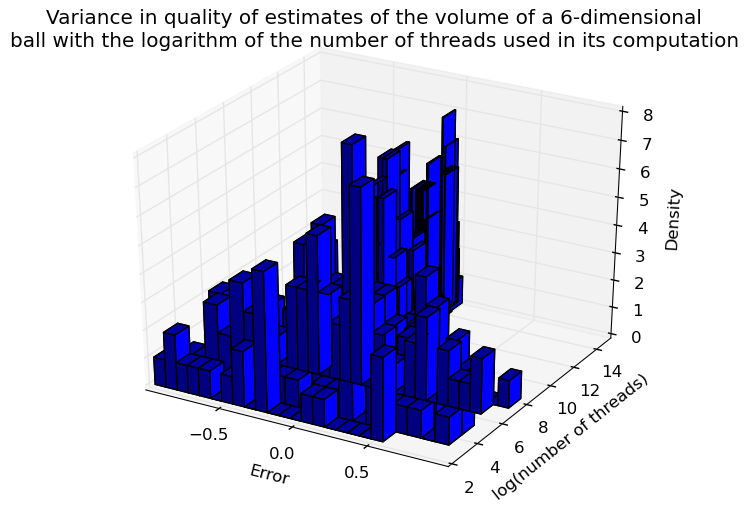
\includegraphics[width = 0.4 \textwidth]{./images/6-dimensions_ball_3d.png}
}
\subfloat[Histograms for the ice cream estimates]{
	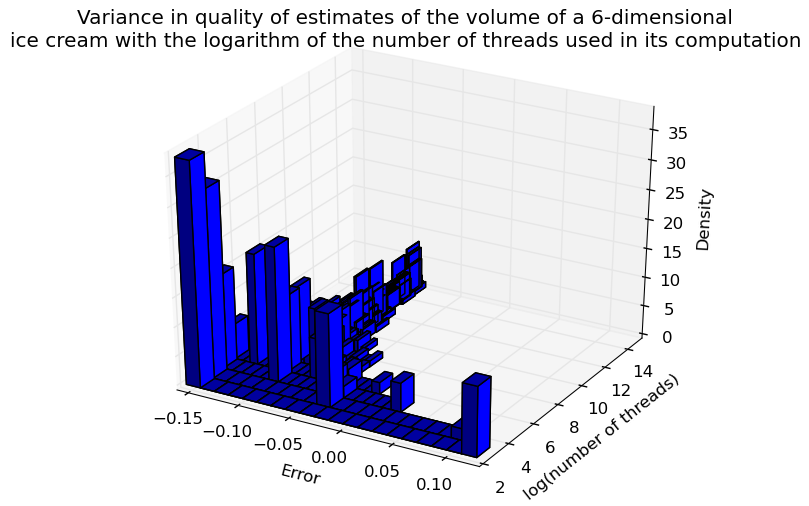
\includegraphics[width = 0.4 \textwidth]{./images/6-dimensions_ice_cream_3d.png}
} 
\\

\subfloat[The worst mistakes made in the ball estimates]{
	\label{fig_2d_ball}
	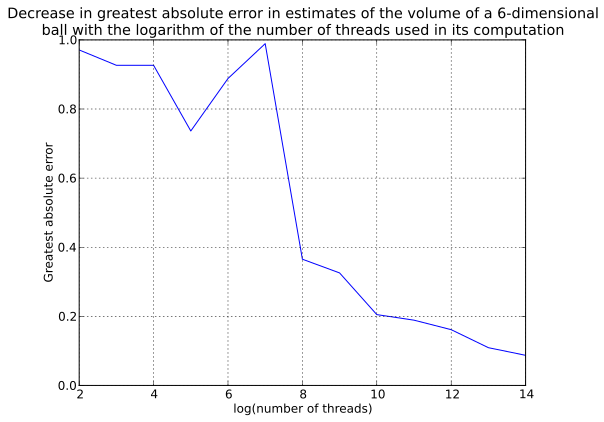
\includegraphics[width = 0.4 \textwidth]{./images/6-dimensions_ball_2d.pdf}
}
\subfloat[The worst mistakes made in the ice cream estimates]{
	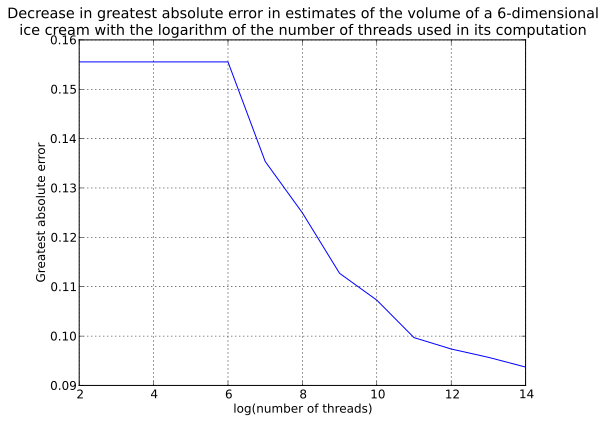
\includegraphics[width = 0.4 \textwidth]{./images/6-dimensions_ice_cream_2d.pdf}
	\label{fig_2d_ice_cream}
}
\label{fig_histograms}
\caption{Variance in errors for various shapes, measured in different ways}
\end{figure}

%Plot minimum number of threads needed for greatest absolute error to drop below 0.2?

So, reading off from figures \ref{fig_2d_ice_cream} and \ref{fig_2d_ball}, in a 6-dimensional ice cream our estimates all become correct for $\varepsilon > 0.1$ for any number of threads greater than $2^11 = 2,048$. For a 6-dimensional ball to within an error of $0.1$, we need more like $2^13 = 8,192$. The papers suggest that at least $400\frac{n\log n}{\varepsilon^2} \approxeq 620,000$ threads are necessary for each stage. Once again, the upper bound is very loose indeed. In all cases, the error drops below $0.2$ for $2^{13}$ threads per stage.

\section{Computation Time for Convex Shapes}\label{sec_time}

It's now time to test the practicalities of this algorithm on a series of convex shape, against already established methods of exact volume computation. The code used for comparison is the same as that used in %cite exact methods
and was run over a series of randomly generated convex shapes. Each shape is the convex hull of the box $[-1,1]^n$, and some variable number of points on the ball of radius $\sqrt n$. We will randomly generate series of shapes in each dimension, increasing the number of points on the hull, and seeing how this affects the time for a volume estimation to complete using the values found above by experimentation

All experiments were conducted on the same hardware and in the same operating system, using the same time metric. The processor is an Intel i5-2500k in a Gigabyte Z68AP-D3 motherboard, connected to 8 GiB of 1,600 MHz dual-channel DDR3 RAM. The programs were both compiled onto a 64-bit install of Ubuntu 12.04 virtualised by Oracle VM Virtualbox with access to 2GiB of RAM. Each time is measured in elapsed clock cycles divided by the number of clocks per second. Using this processor time removes the possibility of error due to other running processes. Neither program is designed to exploit any more than a single processor core, since this would require extensive modification of the code from %cite exact methods
.

Initially, the oracle was implemented with a linear programming solver. A point ${\bm p}$ lies within the convex hull of a set of $v$ vertices $\{{\bm x}^1, {\bm x}^2, {\bm x}^3, ..., {\bm x}^v\}$ iff there exists a vector ${\bm \lambda}$ such that

\begin{align*}
\lambda_1 x^1_1 + \lambda_2 x^2_1 + ... + \lambda_k x^v_1 &= p_1 \\
\lambda_1 x^1_2 + \lambda_2 x^2_2 + ... + \lambda_k x^v_2 &= p_2 \\
&\vdots \\
\lambda_1 x^1_n + \lambda_2 x^2_n + ... + \lambda_k x^v_2 &= p_n \\
\lambda_1 + \lambda_2 + ... + \lambda_v &= 1
\end{align*}

This defines the feasible region of an LP problem, which an LP solver can then inspect to see if any solutions for ${\bm \lambda}$ exist. The solver used was Gurobi, chosen simply because it is the fastest availalbe LP solver. Whilst the LP solver is fast, it will be given vast numbers of LPs to solve, leading to some slow execution times.

This particular method of representing a polytope is known as vertex representation, or v-representation. It is also possible to represent a polytope as two sets of halfspaces. A point lies in a convex polytope iff it is below some set of halfspaces and above some other set of halfspaces. Each halfspace forms one facet of the polytope. Representing a polytop as a set of halfspaces is known as the h-representation. The fastest exact methods require the shape to be converted from v-representation to h-representation before the volume can be computed. Facet enumeration, the problem of performing this computation, is solvable in $O(vl(v,n)f)$ time %http://www.sciencedirect.com/science/article/pii/0925772195000496
, where $f$ is the eventual number of facets, and $l(v,n)$ is the complexity of solving a linear programming problem in $n$ variables and $v$ constraints. Compare this to $O^{*}(n^5l(v,n))$ oracle queries, each being. LP solving is exponential in its worst case,%cite Klee-Minty, "HOW GOOD IS THE SIMPLEX ALGORITHM"
 but is known to be efficient when used against real-world problems. It is also known that when the vertices are generated in this way, on average $f \in \Theta(v)$. In practice, however, I have found facet enumeration to be very slow - slower in fact than estimating a polytope's volume.

Generating a large sample size across several dimensions and several shapes would be very difficult. Where previously we could comfortably generate thousands of data points, here we will have to restrict ourselves to 5 samples from each experiment. In each experiment, we will start with the $n$-dimensional cross-polytope $\{{\bm x} | \sum^n_{i=1}|x_i| \leqslant R\}$, add either 0, 25, 50, 75 or 100 extra vertices, uniformly distributed over the surface of the ball of radius $R$, then estimate the volume of their convex hull. From the definition of the cross-polytope, it is fairly easy to show that it is exactly the convex hull of the points $\pm R{\bm e}_i$ for $i \in \{1,2,...,n\}$, where ${\bm e}_i$ is the vector whose $i^{th}$ component is 1, and all others are 0, so each cross-polytope adds exactly $2n$ vertices to the v-representation. Since $R=\sqrt{n}$, this cross-polytope always contains the unit ball, see Appendix \ref{app_cross_polytope}.

The data will then be passed into an exact solver, which will attempt to convert the shape from its v-representation to an h-representation, then compute the exact volume via the Hybrid Orthomormalisation Technique %cite exact methods
If any stage takes longer than one hour of processor time, it will be terminated early. The number of the experiment will be used as a random number seed; the Mersenne Twister will be seeded from 1, 2, 3, 4, and 5, depending on the experiment, and the Ziggurat will be seeded from a number generated by the Mersenne Twister. Anything that remains unclear can hopefully be explained by reading the code. %cite code


\subsection{A pathological polytope}

Using an LP solver, an oracle query takes time polynomial in the number of verticies in the convex shape. The shape is represented by the vertices on its convex hull, which is referred to as v-representation. The major alternative is the h-representation, in which the shape is represented as a series of halfspaces - one for each facet. It has been proven %http://link.springer.com/content/pdf/10.1007%2FBF01455988.pdf
that the convex hull of $v$ uniformly random vertices from an $n$-ball has, on average, $O(v)$ facets, so either representation is asymptotically equivalent. The probability of hitting a pathological case is sufficiently small that it can justifiably be ignored when considering random inputs, however it is important discuss what would happen in one of these pathological cases.

The moment curve in $\arr^n$ is defined:

$$
\tengm(t) = (t, t^2, t^3, ..., t^n)
$$

A Cyclic Polytope is the convex hull of some sequence of points on $\tengm$. By McMullen's Upper Bound Theorem, a cyclic polytope with $f$ facets has $v$ vertices, with

$$
v = {{f-\lceil n/2 \rceil}\choose{\lfloor {n/2} \rfloor}} + {{f-\lfloor n/2 \rfloor -1} \choose {\lceil {n/2} \rceil - 1}}
$$

Alternatively, a cyclic polytope with $f$ facets has $\Theta(f^{n/2})$ vertices. From this, we can construct a convex hull with an exponential number of both vertices and facets, for which neither representation can be of polynomially bounded size in $n$. No polynomial-time method could be found for testing membership of cyclic polytopes. On this basis, I would call the validity of the assumption of a polynomial time oracle into question. 